\documentclass[a4paper,class=article,border=5pt,tikz]{standalone}


\begin{document}
\begin{tikzpicture}[scale=2]
% draw the horizontal ruler line
\draw [thick] (-0.2,1) -- (5.7cm,1);
% draw centimeter marks with numbers
\foreach \x in {0,1,...,5}{
\draw [very thick] (\x cm,1) -- (\x cm,0.5) node[below,scale=1]{\x};
}
% draw half-centimeter marks
\foreach \x in {0.5,1.5,...,4.5}{
\draw [very thick] (\x cm,1) -- (\x cm,0.75);
}
% draw millimiter marks
\foreach \x in {0.1,0.2,...,5.5}{
\draw [thick] (\x cm,1) -- (\x cm,0.9);
}
% add centimeter label
\node [thick](0,0) {cm};
% add image
\node at (2.34cm,1.9cm)
    {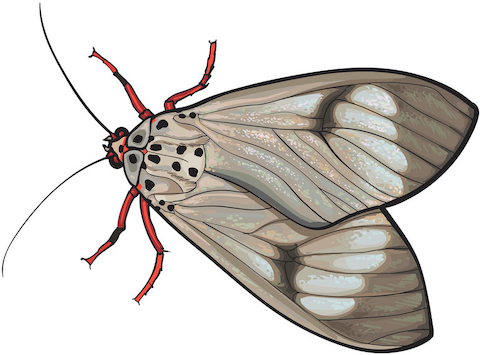
\includegraphics[width=3.9cm,angle=6]{sprint-28-figure-moth}};% size tweaked
% add delimiter lines
\draw [thick, dashed] (1.7,1) -- (1.7,2.7);
\draw [thick, dashed] (3.3,1) -- (3.3,2.7);
\end{tikzpicture}
\end{document}
